\begin{frame}[fragile]{Tutorial: Two-site state optimization}

\begin{columns}

\begin{column}{5cm}

\begin{onlyenv}<1->
\begin{lstlisting}[language=JuliaLocal, style=julia, mathescape, basicstyle=\scriptsize\ttfamily]
$\psi$0 = (Zp1 * Zp2 +
      Zm1 * Zn2)/√2

E($\psi$0) == -1

using Zygote # autodiff

$\partial$E($\psi$) = gradient(E, $\psi$)[1]
norm($\partial$E($\psi$0)) == 2
\end{lstlisting}
\end{onlyenv}

\begin{onlyenv}<2->
\begin{lstlisting}[language=JuliaLocal, style=julia, mathescape, basicstyle=\scriptsize\ttfamily]
$\psi$ = minimize(E, $\partial$E, $\psi$0;
       nsteps=10, $\gamma$=0.1)

E($\psi$0) == -1
E($\psi$) == -1.4142131 $\approx$ -√2
 \end{lstlisting}
\end{onlyenv}

\end{column}

\begin{column}{5cm}

%% \begin{onlyenv}<1-1>
%% |$\psi_0\rangle$ = (|Z+Z+$\rangle$ + \\
%% \ \ \ \ \ \ \ \ \ \ \ |Z-Z-$\rangle$)/√2 \\
%% ~\\
%% $\approx$ -1 \\
%% ~\\
%% Zygote: Julia's automatic \\
%% differentiation library. \\
%% ~\\
%% $\approx$ 2 \\
%% \end{onlyenv}

\begin{onlyenv}<1->
\vspace*{0.0cm}
\begin{center}
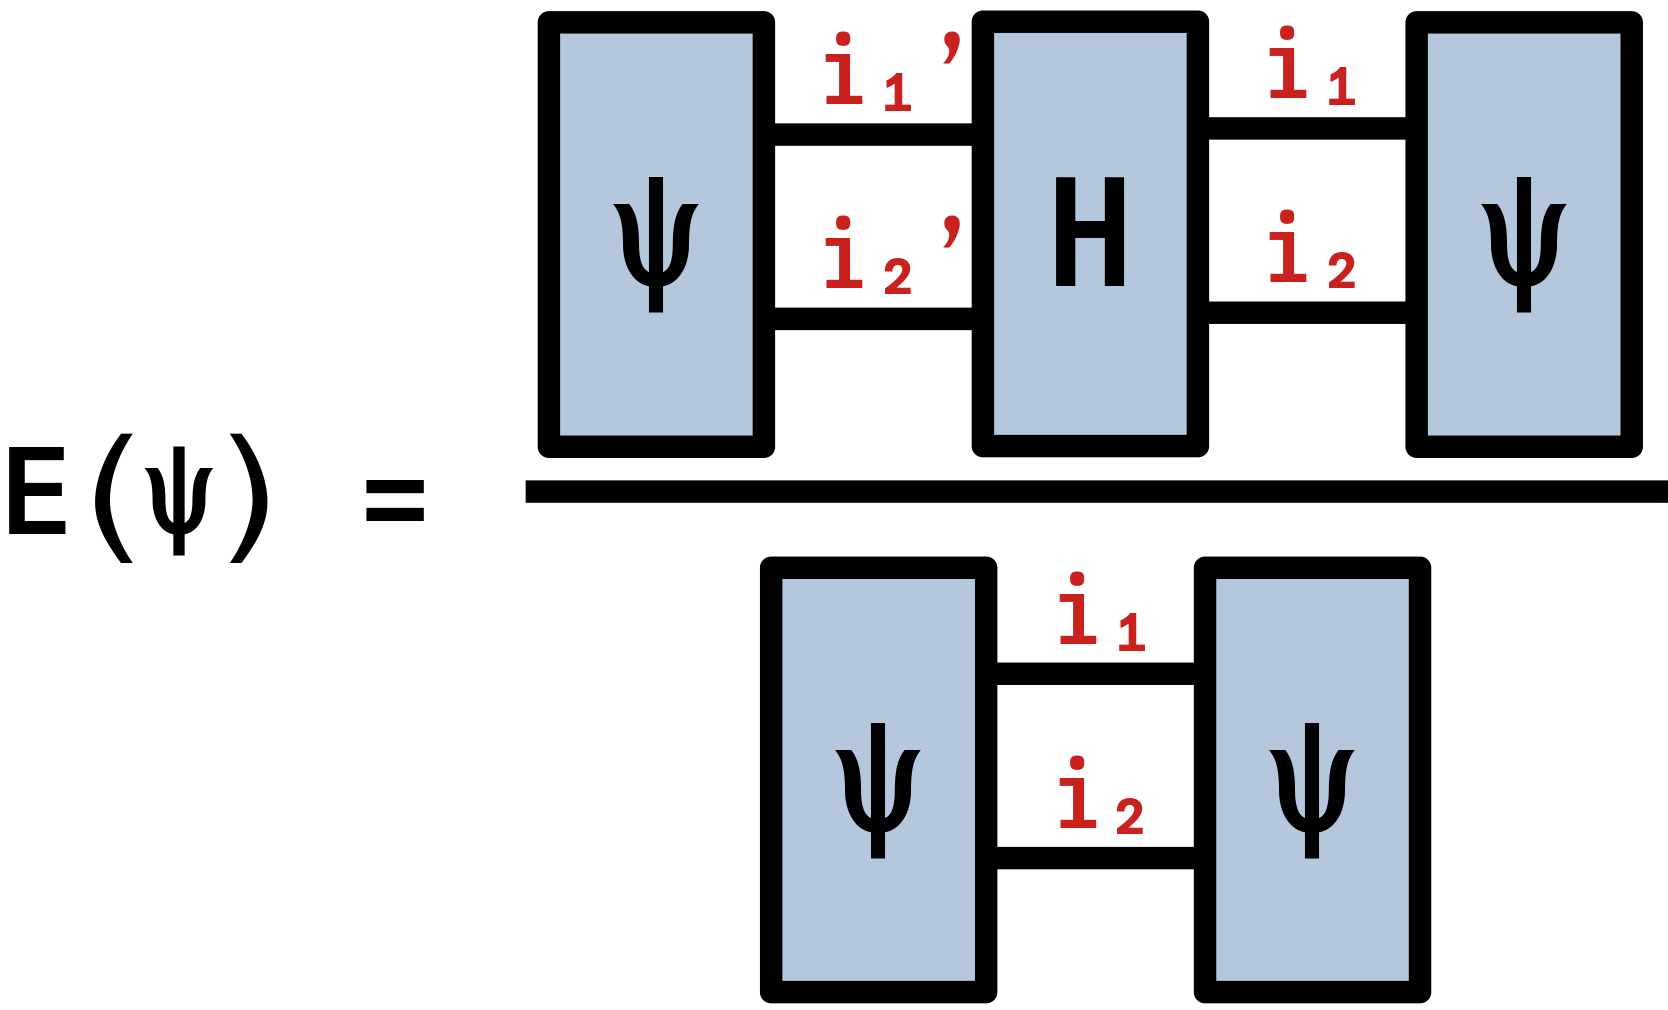
\includegraphics[width=1.0\textwidth]{
  slides/assets/psi12Hpsi12.png
}
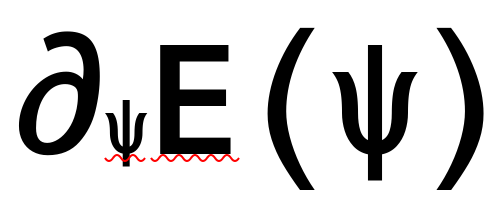
\includegraphics[width=0.3\textwidth]{
  slides/assets/grad_E_psi.png
}
\end{center}
\vspace*{0.0cm}
\end{onlyenv}

\begin{onlyenv}<2->
$\min_{\psi} E(\psi) =$ \\
\ \ \ \ \ $\min_{\psi} \langle\psi|H|\psi\rangle/\langle\psi|\psi\rangle$ \\
~\\
~\\ %(-1, 2) \\
~\\ %(-1.4142131, 0.0010865277) \\
~\\ %\ \ \ \ \ $\approx$ (-√2, 0)
\end{onlyenv}

%% \begin{onlyenv}<3->
%% \vspace*{0.0cm}
%% \begin{center}
%% 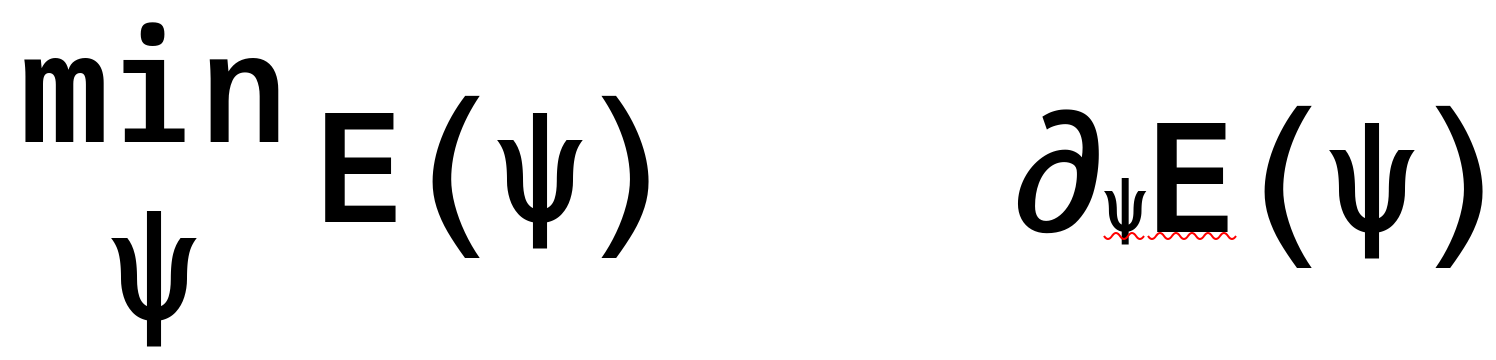
\includegraphics[width=1.0\textwidth]{
%%   slides/assets/min_grad_E_psi.png
%% }
%% \end{center}
%% \vspace*{0.0cm}
%% \end{onlyenv}

\end{column}

\end{columns}

\end{frame}
